\documentclass{beamer}

\mode<presentation>
{
  \usetheme{Madrid}
  \usecolortheme{default}
  \usefonttheme{default}
  \setbeamertemplate{navigation symbols}{}
  \setbeamertemplate{caption}[numbered]
}

\usepackage[portuguese]{babel}
\usepackage[utf8]{inputenc}
\usepackage[T1]{fontenc}
\usepackage{lmodern}
\usepackage{amsmath}
\usepackage{amsfonts}
\usepackage{booktabs}
\usepackage{graphicx}
\usepackage{tikz}
\usetikzlibrary{arrows.meta, positioning}

\title[Análise de Redes Parlamentares]{Arquitetura de Análise de Redes Parlamentares Baseada em Teoria dos Grafos para Identificação de Estruturas de Influência}
\author[Felipe Echeverria Vilhalva]{Felipe Echeverria Vilhalva \\ \vspace{0.5cm} {\small Orientador: Prof.\ Dr.\ Rubens Barbosa Filho}}
\institute[UEMS]{Universidade Estadual de Mato Grosso do Sul (UEMS)}
\date{Novembro de 2026}

\begin{document}

% ============================================================
% 1 — CAPA
% ============================================================
\begin{frame}
  \titlepage
\end{frame}

% ============================================================
\section{Introdução}
% ============================================================

% 2 — MOTIVAÇÃO + CONTRIBUIÇÃO
\begin{frame}{Motivação}
\begin{itemize}
  \item A Câmara dos Deputados produz dezenas de milhares de proposições por ano — mas \textbf{quem colabora com quem?}
  \item Dados de co-autoria legislativa são públicos, porém brutos e de difícil interpretação direta.
  \item A Teoria dos Grafos permite transformar esses dados em \textbf{evidências analíticas} sobre articulação política.
\end{itemize}

\vspace{0.3cm}
\begin{block}{Premissa e contribuição}
A co-autoria parlamentar não é aleatória — reflete alinhamentos políticos e estratégicos. Na esteira de \textbf{Fowler (2006)}, a rede de co-autoria é \textbf{adotada como \textit{proxy} mensurável} de articulação. A contribuição central é a \textbf{arquitetura reprodutível}; a análise 2022--2025 \textbf{demonstra} que ela funciona — não é uma tese política conclusiva.
\end{block}
\end{frame}

% 3 — OBJETIVO GERAL + HIPÓTESE (fundidos)
\begin{frame}{Objetivo e Hipótese}
\textbf{Objetivo geral:} projetar, implementar e validar uma \textbf{arquitetura de software reprodutível} para análise de redes parlamentares, fundamentada na Teoria dos Grafos, capaz de transformar dados legislativos brutos em evidências sobre estruturas de influência na Câmara dos Deputados (2022--2025). \\
\footnotesize \textit{Paradigma:} Design Science Research (DSR) — produção de um \textbf{artefato} validado por rigor de engenharia e teste estatístico. \normalsize

\vspace{0.2cm}
\begin{block}{H1 — Estrutura não-aleatória (única hipótese)}
A modularidade $Q$ da rede é \textbf{significativamente superior} à esperada em grafos nulos ponderados com a mesma sequência de graus.
\end{block}
\begin{alertblock}{H1 é condição de validade, não o clímax}
Antes de ler centralidades e comunidades como influência, é preciso mostrar que a organização modular \textbf{não} é artefato do acaso. As demais análises são \textbf{resultados descritivos complementares}.
\end{alertblock}
\end{frame}

% ============================================================
\section{Fundamentação}
% ============================================================

% 4 — FUNDAMENTAÇÃO TEÓRICA + fórmula do peso (fundidos)
\begin{frame}{Fundamentação Teórica}
\begin{itemize}
  \item \textbf{Grafo bipartido e projeção:} o dataset da Câmara forma $B = (D \cup P,\, E)$ ($D$ = deputados, $P$ = proposições). A rede de co-autoria $G = (D, E', w)$ é a \textbf{projeção unimodal} de $B$ sobre $D$.
  \item \textbf{Centralidades:} grau, intermediação, proximidade e autovetor — cada uma capta uma dimensão distinta de influência.
  \item \textbf{Comunidades:} Louvain (primário) e Label Propagation (contraprova); qualidade medida pela modularidade $Q$.
\end{itemize}

\vspace{0.2cm}
\begin{block}{Peso de aresta — normalização por tamanho do grupo (Newman, 2010)}
\[
  w(i,j) = \sum_{p \,\in\, P_{ij}} \frac{1}{n_p - 1}
\]
\footnotesize $P_{ij}$ = proposições co-autorizadas por $i$ e $j$; \; $n_p$ = nº de autores de $p$. Coautorias em grupos pequenos pesam mais; grandes blocos são atenuados. \normalsize
\end{block}
\end{frame}

% ============================================================
\section{Arquitetura}
% ============================================================

% 5 — ARQUITETURA: PRINCÍPIOS (novo — destaque)
\begin{frame}{Arquitetura — Princípios (Clean Architecture + SOLID)}
\textbf{Contribuição técnica primária do trabalho} (Martin, 2017).

\vspace{0.3cm}
\begin{block}{Regra da Dependência}
Dependências de código apontam \textbf{sempre para dentro}: detalhes de baixo nível (I/O, banco, web) dependem das regras de negócio — nunca o contrário. O núcleo analítico é \textbf{isolado} e testável.
\end{block}

\begin{columns}
\begin{column}{0.5\textwidth}
\textbf{Camadas (círculos concêntricos):}
\begin{itemize}\footnotesize
  \item \textbf{Entidades} — \texttt{models/}
  \item \textbf{Casos de uso} — \texttt{core/}
  \item \textbf{Adaptadores} — \texttt{extraction/}, \texttt{processing/}
  \item \textbf{Drivers} — \texttt{repository/}
\end{itemize}
\end{column}
\begin{column}{0.5\textwidth}
\textbf{SOLID — benefícios:}
\begin{itemize}\footnotesize
  \item Independente de framework
  \item Independente da fonte de dados
  \item Intrinsecamente testável
  \item Extensível a outras casas legislativas
\end{itemize}
\end{column}
\end{columns}
\end{frame}

% 6 — ARQUITETURA: PIPELINE (figura 9 em destaque)
\begin{frame}{Arquitetura — Pipeline de Dados}
\begin{columns}
\begin{column}{0.42\textwidth}
\footnotesize
Fluxo em camadas, cada uma um pacote Python independente:
\vspace{0.2cm}
\begin{itemize}
  \item \textbf{extraction} — download + cache dos CSVs
  \item \textbf{processing} — limpeza, filtros, domínio
  \item \textbf{core} — grafo, centralidades, comunidades
  \item \textbf{repository} — CSV, GEXF, SQLite, JSON
  \item \textbf{visualization} — figuras por ano
\end{itemize}
\end{column}
\begin{column}{0.58\textwidth}
\centering
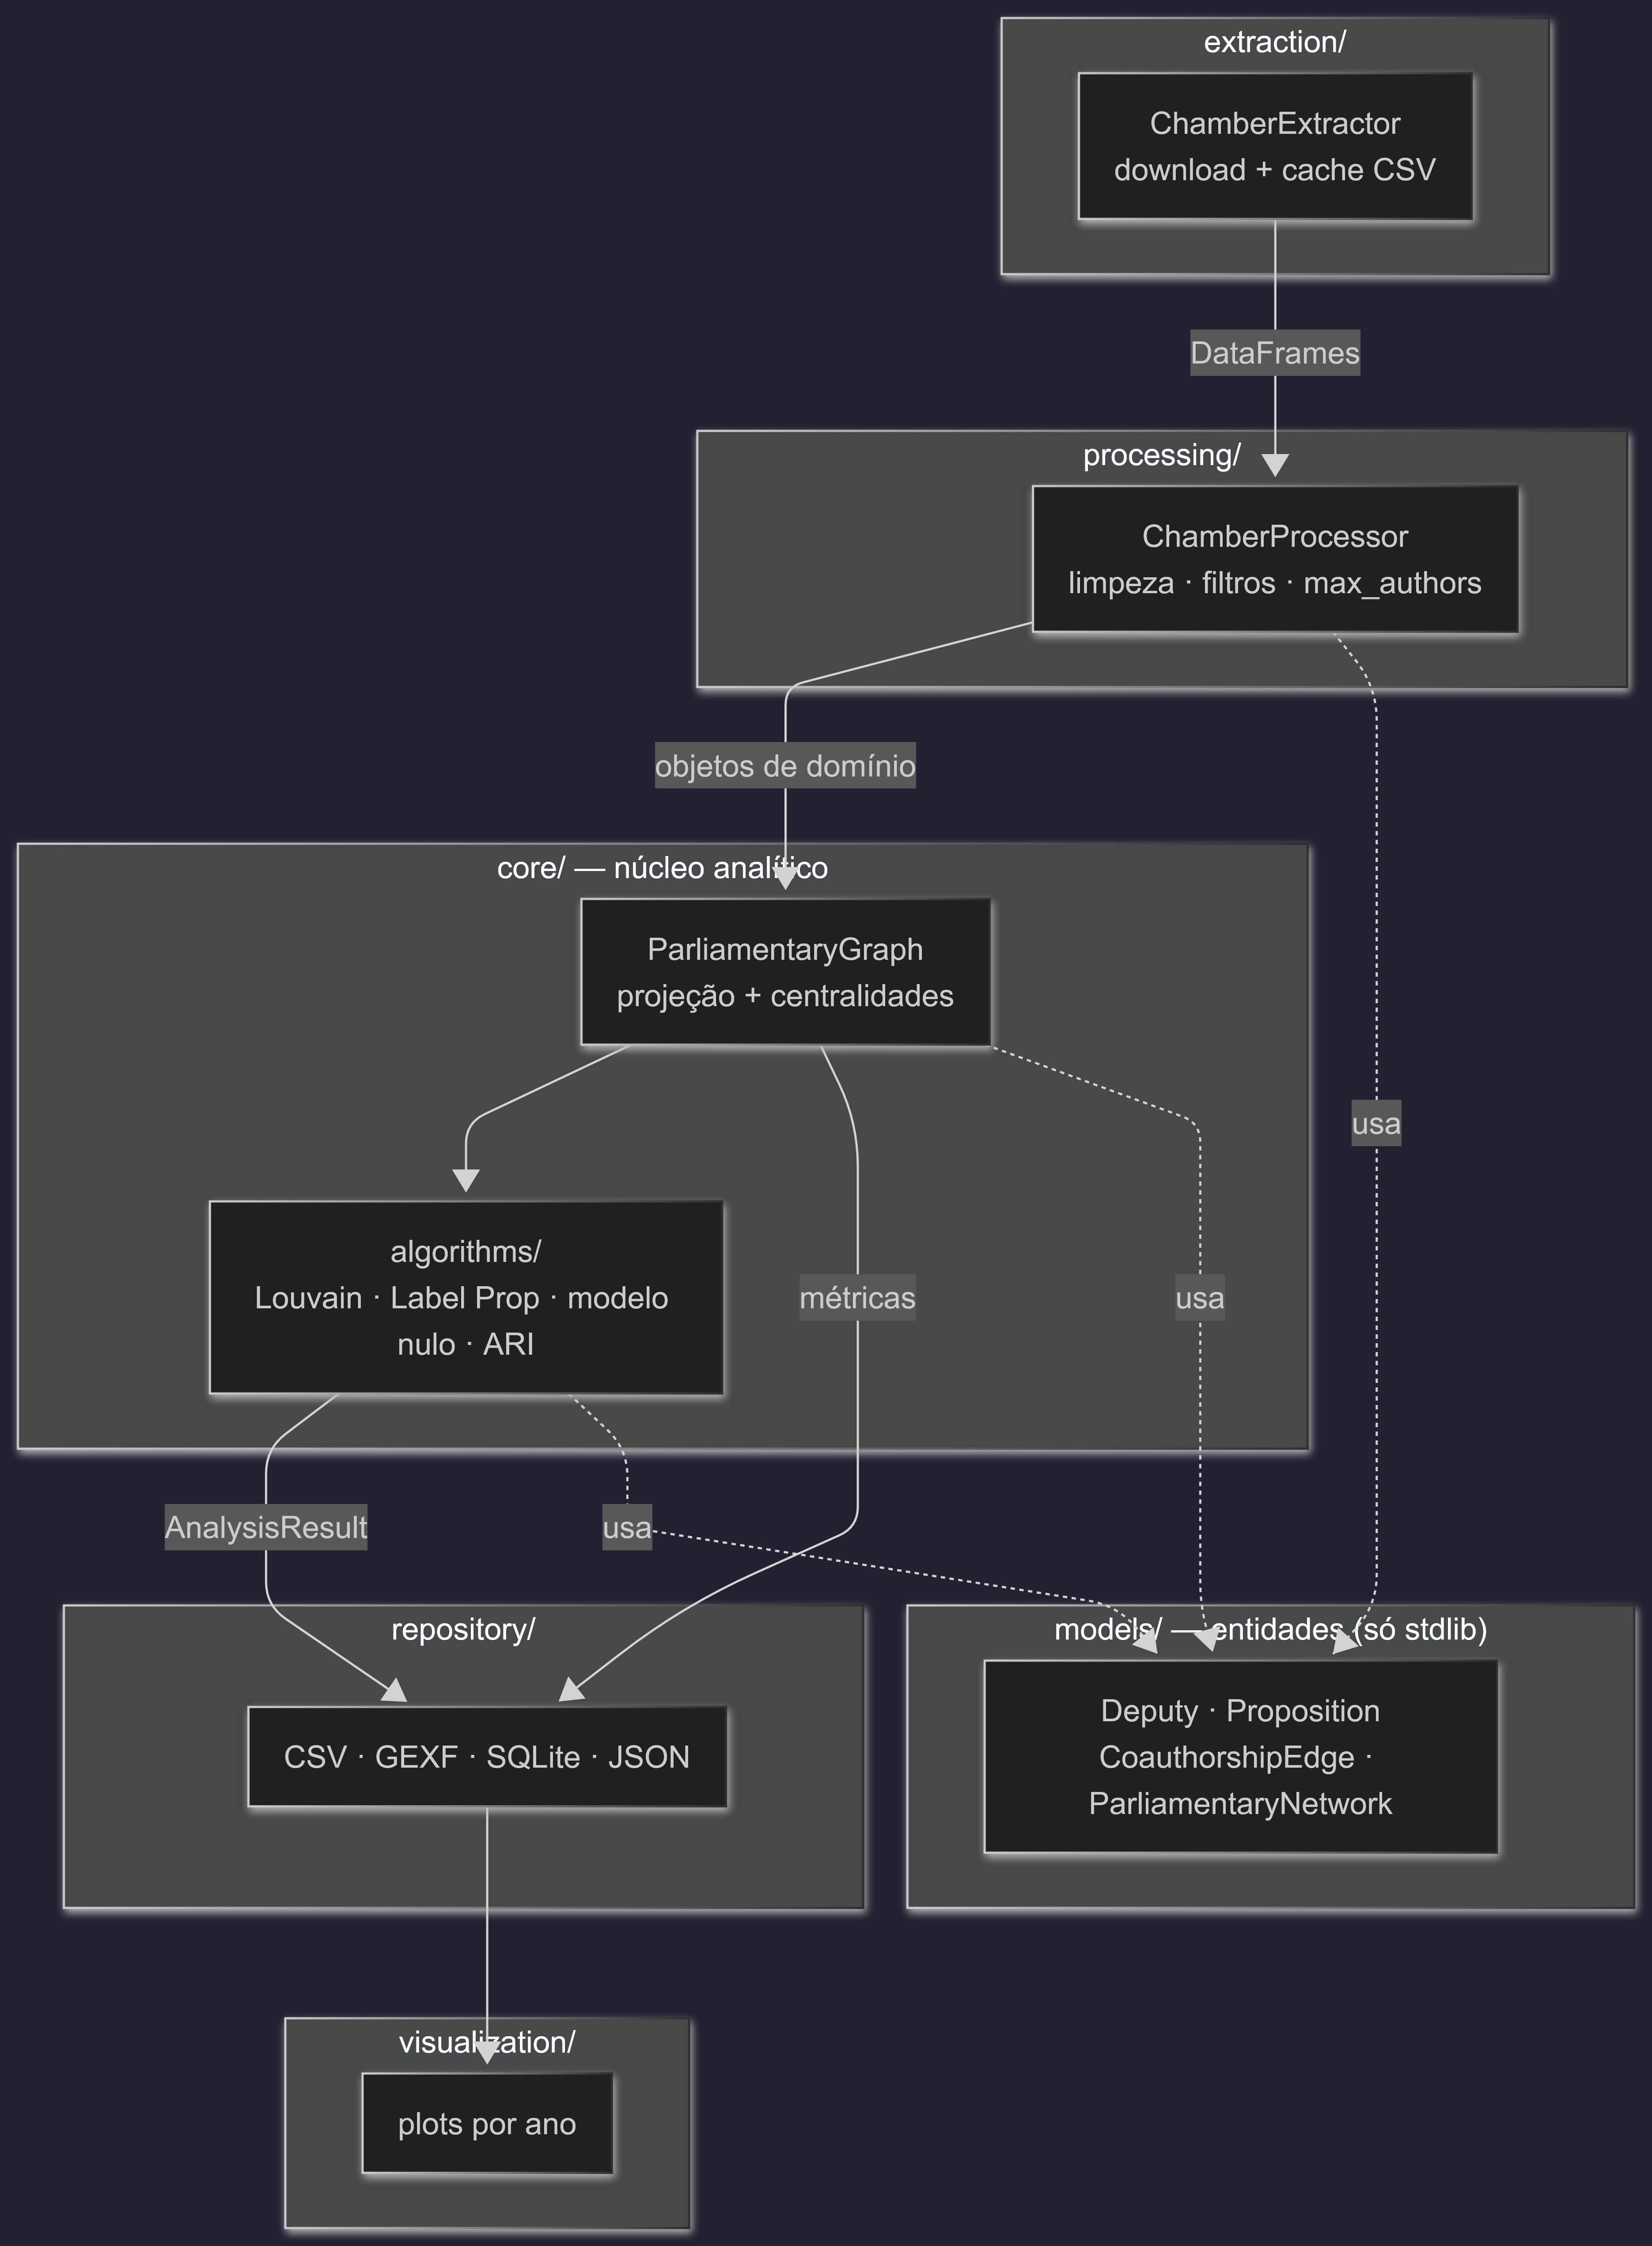
\includegraphics[height=0.82\textheight]{imagens/fig9_pipeline.png}
\end{column}
\end{columns}
\end{frame}

% 7 — ARQUITETURA: QUALIDADE E REPRODUTIBILIDADE (novo — destaque)
\begin{frame}{Arquitetura — Qualidade e Reprodutibilidade}
\begin{block}{Suíte de testes automatizados}
\textbf{217 testes} — cobertura total \textbf{83\%}, núcleo analítico \textbf{$\geq$ 93\%}. Inclui testes unitários, de integração e \textbf{testes de integridade sobre os datasets gerados} (esquema, faixas de valores, coerência CSV $\leftrightarrow$ GEXF).
\end{block}

\begin{block}{Reprodutibilidade estrita}
\begin{itemize}\footnotesize
  \item \textbf{Docker + Docker Compose} — execução completa (4 anos) com \textbf{um único comando}; $\sim$15--25 min.
  \item \textbf{Semente fixa} (\texttt{seed=42}) — execuções idênticas.
  \item \textbf{Validação cruzada:} $Q$ recalculada no Gephi bate com o pipeline.
\end{itemize}
\end{block}

\footnotesize \textbf{Stack:} Python 3.11 · NetworkX 3.2 · Pandas 2.2 · pydantic · pytest \normalsize
\end{frame}

% ============================================================
\section{Metodologia}
% ============================================================

% 8 — DECISÕES METODOLÓGICAS
\begin{frame}{Decisões Metodológicas}
\begin{block}{Filtro de massa de signatários (\textit{ativo} em toda execução)}
Propostas com mais de 30 co-autores são \textbf{excluídas da construção de arestas}. Uma PEC com 226 signatários gera $\approx 25.400$ pares, elevando a densidade a $\sim$85\% — inviabilizando a detecção de comunidades. \textbf{Análise de sensibilidade (limiar 20--40)} confirma que $Q$ é estável e o resultado não depende do valor 30.
\end{block}

\begin{block}{Pesos uniformes por tipo}
Todos os tipos recebem peso igual ($w=1$): sem escala teórica para ponderar PL vs.\ PEC. A seleção qualitativa fica no \textbf{filtro de tipos} (PL, PEC, PLP, PDL, EMC).
\end{block}

\begin{block}{Representação das centralidades}
Grau e autovetor \textbf{ponderados}; intermediação e proximidade \textbf{topológicas} (o peso codifica intensidade, não distância).
\end{block}
\end{frame}

% 9 — VALIDAÇÃO POR MODELO NULO (método + resultado fundidos)
\begin{frame}{Validação por Modelo Nulo — Teste de H1}
\begin{block}{Teste de permutação (200 grafos nulos, $\alpha = 0{,}05$)}
\textit{Double-edge-swap} preserva a sequência de graus; os \textbf{pesos originais são reatribuídos} às arestas reconfiguradas — nulo \textbf{ponderado e homogêneo} com $Q_{\text{obs}}$. \\
$p$-valor via estimador aditivo (North et al., 2002): $p = (r+1)/(m+1)$.
\end{block}

\vspace{0.2cm}
\begin{center}
$Q_{\text{obs}} = 0{,}634 \;>\; Q_{\text{nulo}} = 0{,}467 \pm 0{,}005 \qquad p < 0{,}005 \;\Rightarrow\; \textbf{SIGNIFICATIVO}$
\end{center}
\vspace{0.2cm}

\begin{itemize}\footnotesize
  \item \textbf{Nenhum} dos 200 grafos nulos atingiu $Q \geq Q_{\text{obs}}$.
  \item \textbf{H1 confirmada nos 4 anos} (2022--2025), $p < 0{,}005$ — estrutura não emerge por acaso.
\end{itemize}
\end{frame}

% ============================================================
\section{Resultados}
% ============================================================

% 10 — MÉTRICAS DA REDE 2025
\begin{frame}{Métricas da Rede — 2025}
\begin{table}
\centering
\small
\begin{tabular}{lr}
\toprule
\textbf{Métrica} & \textbf{Valor} \\
\midrule
Nós na rede (co-autores ativos) & 331  \\
Arestas (co-autorias únicas)    & 5.407  \\
Densidade                       & 9,90\% \\
Componentes conexos             & 6 \\
Componente principal            & 319 nós (96,4\%) \\
Modularidade Louvain ($Q$)      & 0,634 \\
Comunidades (Louvain / Label Prop.) & 16 / 10 \\
ARI (Louvain $\times$ Label Prop.)  & 0,423 \\
\bottomrule
\end{tabular}
\end{table}
\end{frame}

% 11 — FIGURA 13: COMUNIDADES vs PARTIDOS (imagem grande)
\begin{frame}{Comunidades $\times$ Partidos — Rede de 2025}
\begin{columns}
\begin{column}{0.5\textwidth}
\centering
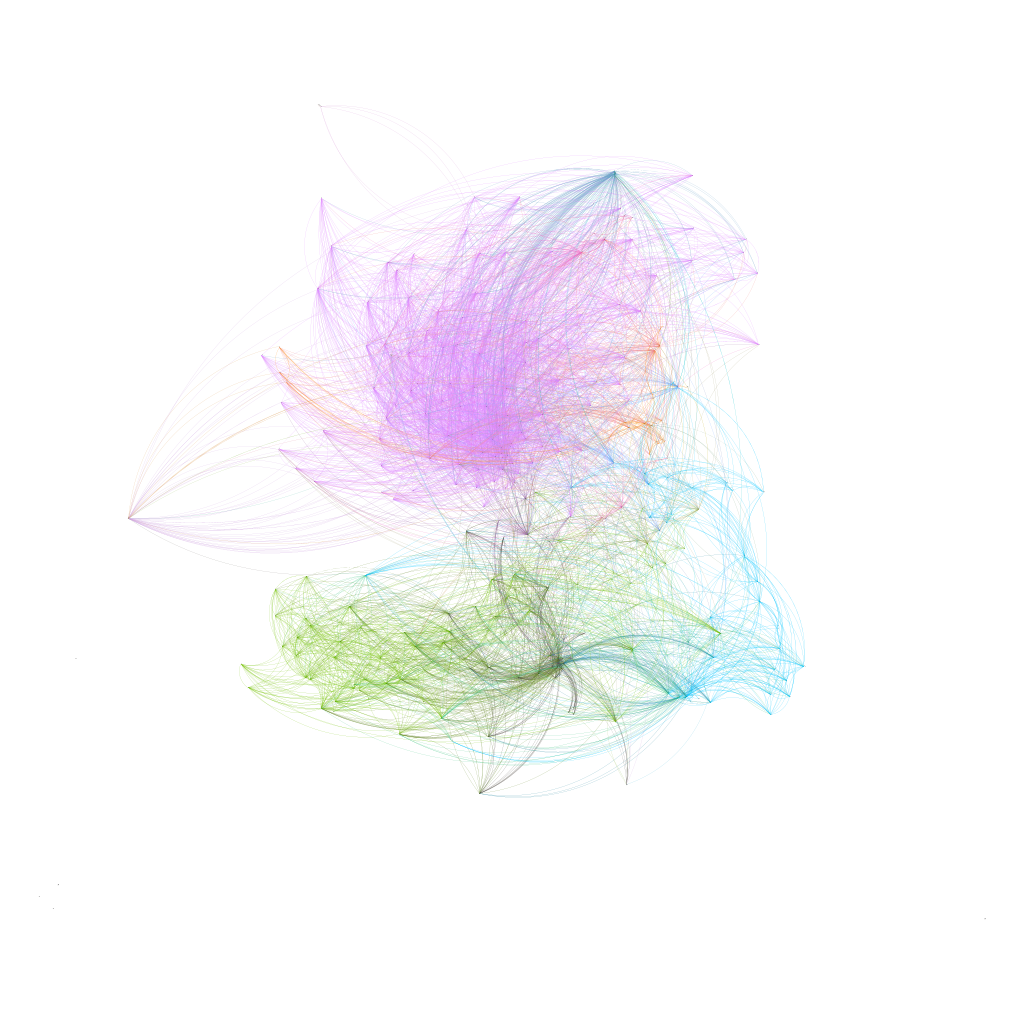
\includegraphics[width=\textwidth]{imagens/fig13_panel0.png}\\
\footnotesize (a) Cor por comunidade (Louvain)
\end{column}
\begin{column}{0.5\textwidth}
\centering
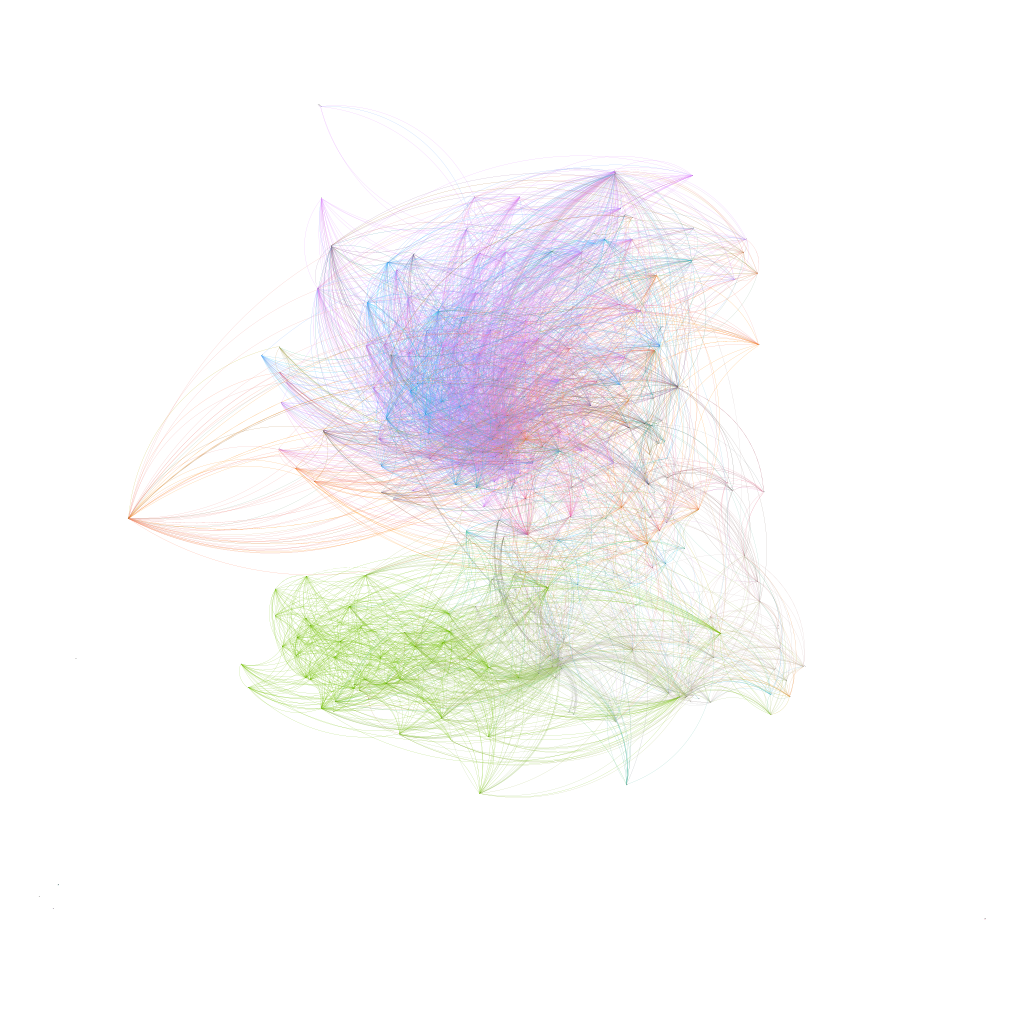
\includegraphics[width=\textwidth]{imagens/fig13_panel1.png}\\
\footnotesize (b) Cor por filiação partidária
\end{column}
\end{columns}
\vspace{0.2cm}
\footnotesize \centering Mesmo \textit{layout} ForceAtlas 2 (só arestas). A concordância espacial confirma que as comunidades \textbf{recuperam a organização partidária} — no nível de coalizão.
\end{frame}

% 12 — FIGURA 14: EVOLUÇÃO TEMPORAL
\begin{frame}{Estabilidade Temporal (2022--2025)}
\centering
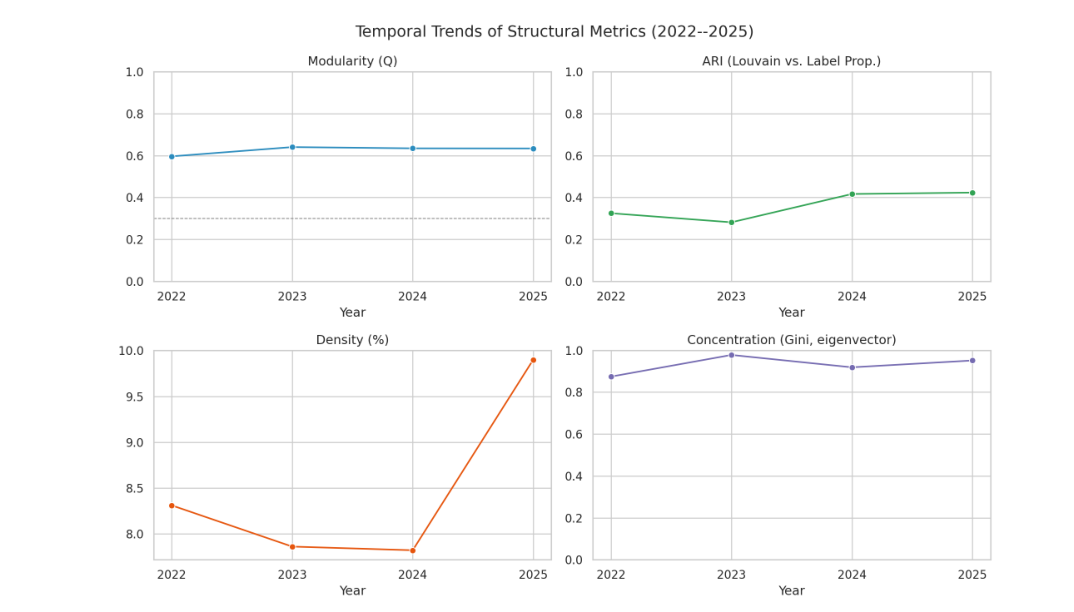
\includegraphics[width=0.92\textwidth]{imagens/fig14_temporal.png}

\vspace{0.1cm}
\footnotesize O padrão é \textbf{persistente}: $Q \in [0{,}596;\,0{,}640]$ acima do patamar significativo (0,3) nos 4 anos; concentração no autovetor sempre alta (Gini $>$ 0,87). H1 sobrevive à transição de legislatura (56ª $\to$ 57ª).
\end{frame}

% 13 — DEPUTADOS DE DESTAQUE + INTERPRETAÇÃO
\begin{frame}{Deputados de Destaque — 2025}
\begin{columns}
\begin{column}{0.5\textwidth}
\footnotesize \textbf{Top \textit{betweenness}} (pontes)
\begin{enumerate}\footnotesize
  \item Franciane Bayer (REPUBLIC)
  \item Alberto Fraga (PL)
  \item Bibo Nunes (PL)
  \item Pezenti (MDB)
  \item Evair Vieira de Melo (PP)
\end{enumerate}
\end{column}
\begin{column}{0.5\textwidth}
\footnotesize \textbf{Top \textit{weighted degree}} (coesão)
\begin{enumerate}\footnotesize
  \item Célia Xakriabá (PSOL)
  \item Adriana Ventura (NOVO)
  \item Fernanda Melchionna (PSOL)
  \item Marcel van Hattem (NOVO)
  \item Luiz Lima (PL)
\end{enumerate}
\end{column}
\end{columns}

\vspace{0.2cm}
\begin{alertblock}{Articulação $\neq$ poder institucional}
Pontes se distribuem por vários partidos — o principal \textit{broker} \textbf{não} é do maior bloco. Já o grau ponderado é dominado por partidos pequenos e coesos (PSOL, NOVO): \textbf{câmaras de eco}. A rede mede \textbf{quem articula}, não quem controla pauta ou relatorias.
\end{alertblock}
\end{frame}

% ============================================================
\section{Conclusão}
% ============================================================

% 14 — CONCLUSÃO + TRABALHOS FUTUROS (fundidos)
\begin{frame}{Conclusão e Trabalhos Futuros}
\begin{block}{Conclusão}
\begin{itemize}\footnotesize
  \item \textbf{Artefato modular e reprodutível} entregue (Docker, 217 testes, código aberto) — a contribuição central.
  \item \textbf{H1 confirmada} nos 4 anos com validação estatística robusta ($p < 0{,}005$).
  \item Centralidades e comunidades \textbf{caracterizam} as estruturas de influência: coalizões, pontes e a distinção articulação $\neq$ poder.
\end{itemize}
\end{block}

\begin{block}{Trabalhos futuros}
\begin{itemize}\footnotesize
  \item \textbf{Cruzamento com votação nominal:} testar se a co-autoria prediz votos.
  \item Extensão da série histórica (ex.: 2010--2025) e análise longitudinal.
  \item Algoritmo de \textbf{Leiden}; inclusão das emendas (EMC) na estrutura.
  \item \textbf{Redes Neurais de Grafos (GNNs)} para predição de comportamento legislativo.
\end{itemize}
\end{block}
\end{frame}

% 15 — OBRIGADO
\begin{frame}
  \centering
  \vspace{1cm}
  {\Large \textbf{Obrigado!}}\\[1cm]
  \textit{Felipe Echeverria Vilhalva}\\
  \textit{Orientador: Prof.\ Dr.\ Rubens Barbosa Filho}\\[0.5cm]
  \small
  Repositório: \texttt{github.com/fvilhalva/parliament-graph-architecture}\\[0.3cm]
  \textit{Dados: Portal de Dados Abertos da Câmara dos Deputados}
\end{frame}

\end{document}